%\documentclass[12pt,notes]{beamer}       % print frame + notes
%\documentclass[12pt,notes=only]{beamer}   % only notes
\documentclass[12pt]{beamer}              % only frames
\usetheme{Madrid}
\usepackage[utf8]{inputenc}
\usepackage[english,german]{babel}
\usepackage[T1]{fontenc}
\usepackage{amsmath}
\usepackage{amsfonts}
\usepackage{amssymb}
\usepackage{graphicx}
\usepackage[style=authortitle-icomp,backend=biber]{biblatex}
\usepackage[babel,german=guillemets]{csquotes}
\addbibresource{seminararbeit_monitoring.bib}
\makeindex
\author{Markus Österle}
\title{Servermonitoring im Rechenzentrum}
%\subtitle{am Beispiel von Linux Servern}
%\setbeamercovered{transparent} 
%\setbeamertemplate{navigation symbols}{} 
%\logo{} 
%\institute{} 
\date{18. Januar 2016} 
\subject{Präsentation zur Seminararbeit im Studiengang \glqq Verwaltungsinformatik\grqq} 
\begin{document}
\begin{frame}
\titlepage
\end{frame}

%\begin{frame}
%\tableofcontents
%\end{frame}

\begin{frame}{Übersicht - roter Faden}
\begin{itemize}
	\item Monitoring was ist das eigentlich? - Definitionen
	\item Warum Monitoring?
	\item Was wird überwacht?
	\item Wie wird es gemacht? - verwendete Software
\end{itemize}
\end{frame}
\note[itemize]{
	\item point 1
	\item point 2
}
\begin{frame}{Monitoring}
	%TODO: Hier lt. Duden oder korrektes Zitat?
	Laut \cite[S. 701; Stichwort Monitoring]{duden}: \\
	
	\begin{center}
		\glqq [Dauer]beobachtung (eines bestehenden Systems)\grqq
	\end{center}
	
\end{frame}
\begin{frame}{Arten des Monitorings}
	\begin{itemize}
		\item proaktives Monitoring
		\item reaktives Monitoring
		\item SLA Monitoring
	\end{itemize}
\end{frame}
%TODO Warum Monitoring hier oder unten?
\begin{frame}{Proaktives Monitoring}
	\begin{center}
		Monitoring, bei dem versucht wird, Event-Muster zu ermitteln, um mögliche zukünftige Ausfälle zu prognostizieren.
	\end{center}
	 
\end{frame}
\begin{frame}{Reaktives Monitoring}
	\begin{center}
		Monitoring, das als Reaktion auf ein bestimmtes Event entsprechende Maßnahmen einleitet. Beispielsweise die Auslösung eines Batchjobs, sobald ein vorheriger Batchjob abgeschlossen wurde, oder die Erfassung eines Incident, wenn ein Fehler auftritt. 
	\end{center}
\end{frame}
\begin{frame}{SLA Monitoring}
	\underline{Service Level Agreement (SLA):}\medskip
	
	Vereinbarung zwischen IT-Dienstleister und Kunde\bigskip
	
	%Grundsatz: 
	%Niemals ein SLA vereinbaren, dass man nicht messen kann
	%Niemals ein SLA vereinbaren, dessen Leistungserbringung nicht im eigenen Verantwortungsbereich liegt
	\underline{SLA Monitoring:}\medskip
	
	Überwacht die Einhaltung der im SLA festgelegten Kennzahlen (Verfügbarkeit, Zuverlässigkeit, Durchsatz, Antwortzeiten) nach den vereinbarten Messkriterien innerhalb der vereinbarten Zeiten.
\end{frame}
\begin{frame}{Warum Monitoring?}
	\begin{itemize}
		\item standardisierte Prozesse/Abläufe
		\item Schutz vor Systemausfällen
		\item Überblick über den Systemstatus
		\item Nachweis von Verfügbarkeit
		\item Reporting
	\end{itemize}
\end{frame}
\begin{frame}{Was wird überwacht?}
	\begin{center}
		\begin{itemize}
			\item Grundlegende Überwachung
			\begin{itemize}
				\item Erreichbarkeit
				%Alle Serverdienste erreichbar, Server erreichbar, Netzwerk soweit ok
			\end{itemize}
			\item Erweiterte Überwachung
			\begin{itemize}
				\item Auslastung
				\item freier Speicherplatz
			\end{itemize}
			\item Spezialisierte Überwachung
			\begin{itemize}
				\item Temperatur im Serverraum
				\item Stromversorgung
				%Hierfür wird individuell Hard- und Software nötig
			\end{itemize}
		\end{itemize}
	\end{center}
	
	
\end{frame}
\begin{frame}{Wie wird überwacht?}
	\begin{itemize}
		%TODO Was heißt SAR
		%iotop -> Festplatten, htop -> grafisch schickeres top, volle Ausgabe der laufenden Prozesse mit allen Optionen, atop -> Advanced top, ntop -> top fürs Netzwerk
		\item Bordmitteln (sysstat-Paket (sar, iostat), top und seine Derivate)
		%Linux hat große Mengen Tools dabei um viele sinnvolle Werte aus dem System zu bekommen. Das Sysstat - Paket mit der Möglichkeit Performancedaten über SAR sogar historisch schreiben zu lassen oder TOP mit seinen Derivaten (atop, htop, iotop)
		\item zentrale Monitoring-Lösung
		\begin{itemize}
			\item proprietäre Lösung
			%CA Unified Infrastructure Management
			\item Cacti
			\item Nagios \& Derivate
		\end{itemize}
	\end{itemize}
	
\end{frame}
\begin{frame}{Warum Nagios?}
	\begin{itemize}
		\item Mächtiges und modular erweiterbares Tool
		\item Kann nahezu alle verfügbaren IT-System überwachen
		%inkl. Android...
		\item freie Software unter der GPL Lizenz
		%GPLv2
		\item keine Lizenzkosten
	\end{itemize}
\end{frame}
%\begin{frame}{Nagios Historie}
%	1996 als simple Ping Check Lösung 
%	seit 1999 auf dem Markt, zuerst als Netsaint
%	%TODO rekursives Acronym erklären -> Zettel
%	rekursives Acronym
%\end{frame}
\begin{frame}{Nagios - Aufbau}
	%TODO Aktive/Passive Checks was ist das...
	%Aktiv: in regelmäßigen definierten Abständen werden Programme ("checks") aufgerufen, die ein Überprüfung durchführen, Rückgabewerte werden ausgewertet, besteht ein Fehler über eine bestimmte Zeit wechselt der Status und es wird eine Benachrichtigung verschickt
	%Passiv: Ein Dienst meldet einen Fehler, die Meldung wird ausgewertet, die zuständige Person wird informiert.
	\begin{figure}
		\centering
		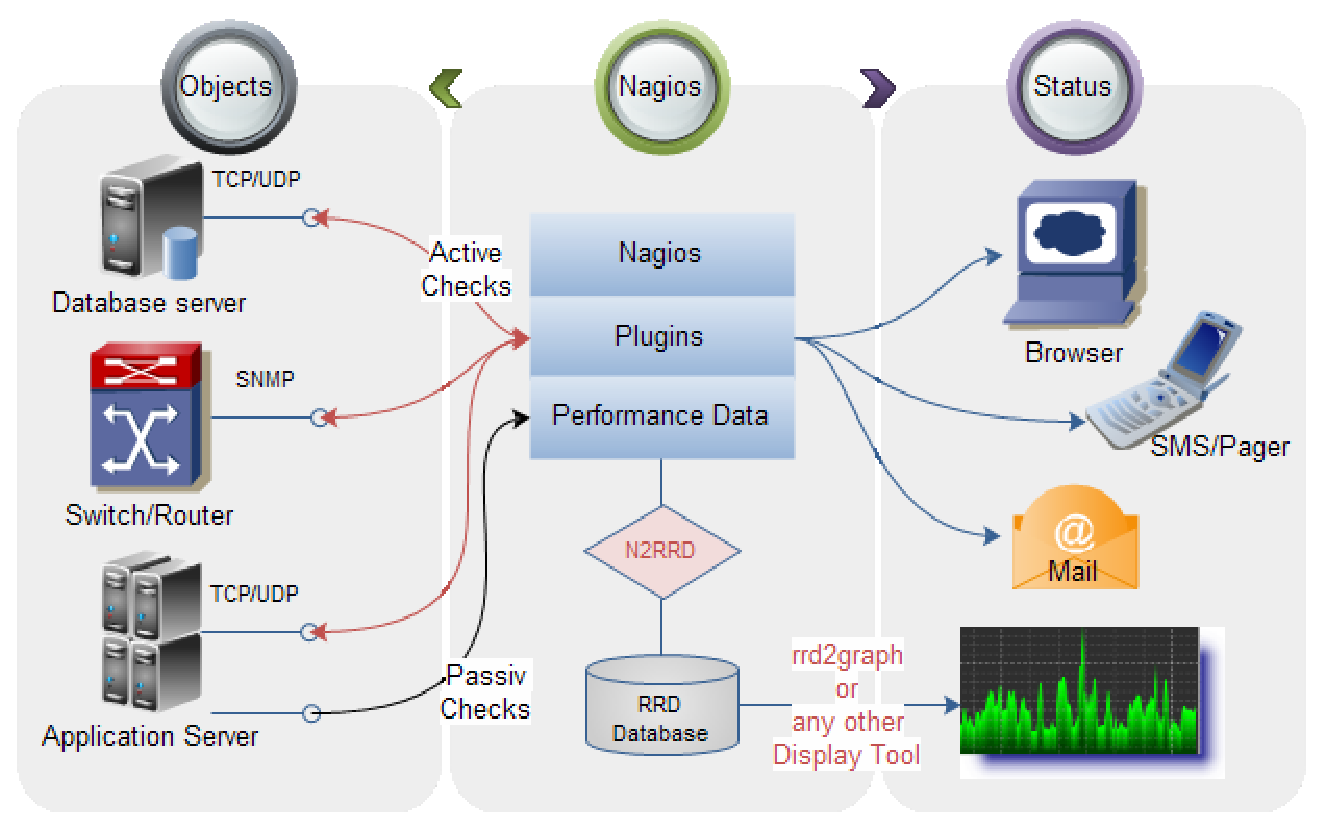
\includegraphics[width=0.9\textwidth]{pics/NagiosMonitoring.eps}
		\caption[Grober Aufbau von Nagios]{Aufbau einer Nagios Appliance - Quelle: \textcite{nagiosaufbau}}
	\end{figure}
\end{frame}
\begin{frame}{Nagios - Probleme}
	\begin{itemize}
		\item Mächtiges modular erweiterbares Tool
		\item Für eine Grundkonfiguration ist schon einiges an Wissen notwendig
	\end{itemize}
\end{frame}
\begin{frame}{Check\_MK - die Lösung}
	%Brot & Butter Monitoring
	\begin{figure}
		\centering
		\includegraphics[width=1\textwidth]{pics/Check_MK_Screen.eps}
		\caption[Check\_MK]{Check\_MK}
	\end{figure}
\end{frame}
\begin{frame}{Check\_MK - Aufbau}
	\begin{figure}
		\centering
		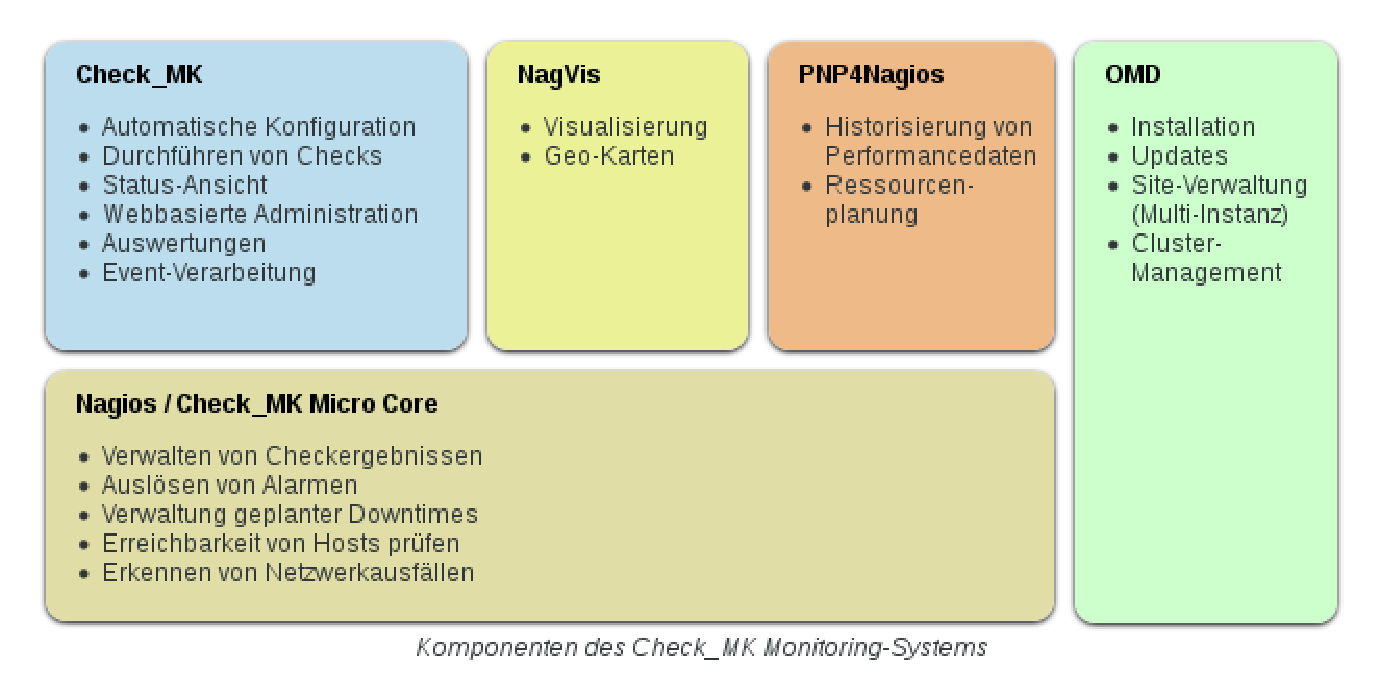
\includegraphics[width=1\textwidth]{pics/checkMKAufbau.eps}
		\caption[Komponenten des Check\_MK Monitoring Systems]{Komponenten des Check\_MK Monitoring Systems (Quelle: \textcite{checkmkmonitoringpic})}
	\end{figure}
\end{frame}
\begin{frame}{Fürs Protokoll: Ein Elch - Elasticsearch - Logstash - Kibana}
\begin{figure}
		\centering
		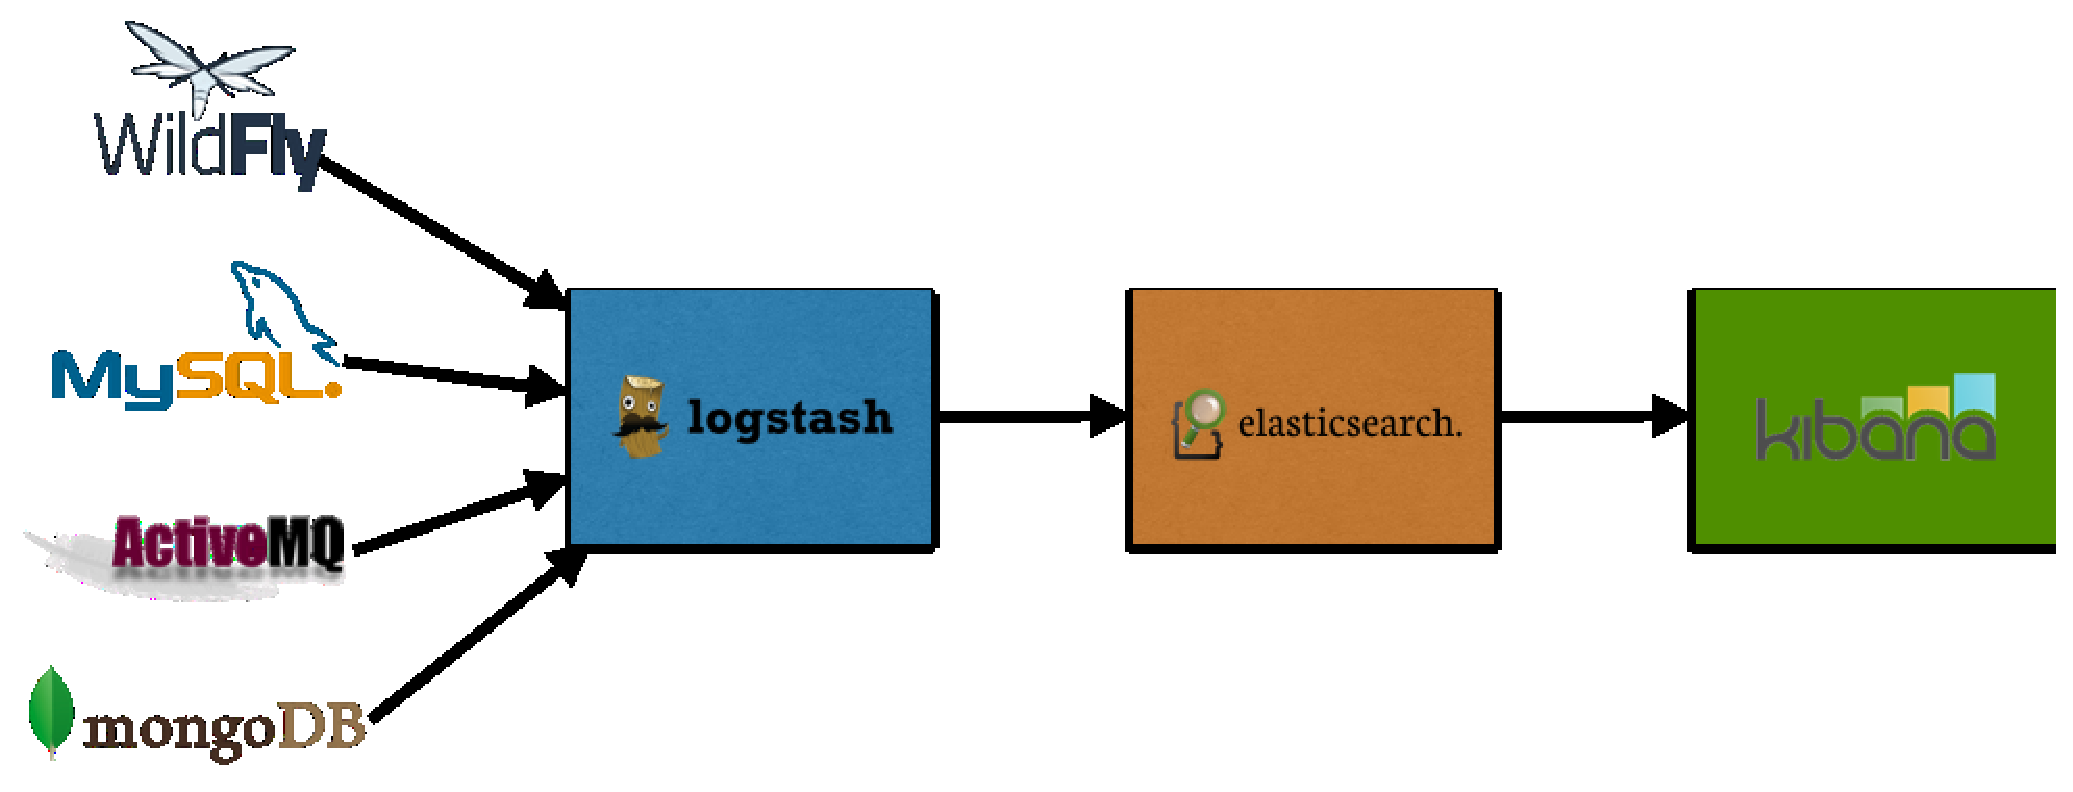
\includegraphics[width=1\textwidth]{pics/elk-stack.eps}
		\caption[Aufbau eines Elasticsearch - Logstash - Kibana Stacks]{Aufbau eines Elasticsearch - Logstash - Kibana Stacks (Quelle: \textcite{elkstackpic})}
	\end{figure}
\end{frame}
\begin{frame}{Quellen}
	\printbibliography
\end{frame}
\begin{frame}{Ende}
	\begin{center}
	Danke für Eure die Aufmerksamkeit!
	\end{center}
	
\end{frame}
\end{document}